\documentclass[12pt,a4paper]{article}

% ─── Page Layout ───────────────────────────────────────────────────────────────
\usepackage[a4paper, margin=0.8in, headheight=14pt]{geometry}

% ─── Fonts (XeLaTeX) ───────────────────────────────────────────────────────────
\usepackage{fontspec}
\usepackage{unicode-math}
\setmainfont{TeX Gyre Pagella}
\setmonofont[Scale=0.88]{TeX Gyre Cursor}
\setmathfont{Latin Modern Math}

% ─── Packages ──────────────────────────────────────────────────────────────────
\usepackage{xcolor}
\usepackage{colortbl}
\usepackage{titlesec}
\usepackage{enumitem}
\usepackage{tabularx}
\usepackage{booktabs}
\usepackage{array}
\usepackage{amsmath}
\usepackage{tikz}
\usetikzlibrary{shapes.geometric, arrows.meta, positioning, calc, fit, decorations.pathreplacing}
\usepackage{tcolorbox}
\tcbuselibrary{skins, breakable}
\usepackage{hyperref}
\usepackage{fancyhdr}
\usepackage{graphicx}
\usepackage{microtype}
\hyphenpenalty=10000
\exhyphenpenalty=10000
\sloppy
\usepackage{caption}
\usepackage{setspace}
\usepackage{multirow}
\usepackage{tocloft}

% ─── Q&A helper ────────────────────────────────────────────────────────────────
\newcommand{\Q}[1]{\textbf{#1}\par\noindent\ignorespaces}

% ─── Colour Palette ────────────────────────────────────────────────────────────
\definecolor{myred}{RGB}{196,30,58}
\definecolor{mydark}{RGB}{30,30,50}
\definecolor{mygreen}{RGB}{14,120,80}
\definecolor{myteal}{RGB}{0,130,140}
\definecolor{myamber}{RGB}{180,100,0}
\definecolor{mypurple}{RGB}{100,30,160}
\definecolor{mygray}{RGB}{246,247,249}
\definecolor{mgframe}{RGB}{180,185,200}
\definecolor{watermark}{RGB}{145,150,170}
\definecolor{hdrred}{RGB}{250,232,235}
\definecolor{hdrgreen}{RGB}{220,244,233}
\definecolor{hdrteal}{RGB}{220,242,244}
\definecolor{hdramber}{RGB}{253,242,215}
\definecolor{hdrpurple}{RGB}{238,228,255}
\definecolor{hdrgray}{RGB}{238,240,245}
\definecolor{rowalt}{RGB}{250,251,253}

% ─── Section Formatting ────────────────────────────────────────────────────────
\titleformat{\section}
  {\large\bfseries\color{myred}}{\thesection.}{0.5em}{}
  [\vspace{1pt}{\color{myred}\rule{\linewidth}{0.8pt}}]
\titleformat{\subsection}
  {\normalsize\bfseries\color{myteal}}{\thesubsection}{0.5em}{}
\titlespacing*{\section}{0pt}{18pt}{7pt}
\titlespacing*{\subsection}{0pt}{11pt}{4pt}

% ─── Paragraph ─────────────────────────────────────────────────────────────────
\setlength{\parindent}{0pt}
\setlength{\parskip}{4pt}

% ─── TOC Styling ───────────────────────────────────────────────────────────────
\renewcommand{\cfttoctitlefont}{\large\bfseries\color{myred}}
\renewcommand{\cftaftertoctitle}{\par\noindent{\color{myred}\rule{\linewidth}{0.8pt}}}
\setlength{\cftbeforetoctitleskip}{0pt}
\setlength{\cftaftertoctitleskip}{6pt}
\renewcommand{\cftsecfont}{\normalsize\bfseries\color{mydark}}
\renewcommand{\cftsecpagefont}{\normalsize\bfseries\color{mydark}}
\renewcommand{\cftsecleader}{\cftdotfill{\cftdotsep}}
\setlength{\cftbeforesecskip}{7pt}
\renewcommand{\cftsubsecfont}{\small\color{mydark}}
\renewcommand{\cftsubsecpagefont}{\small\color{mydark}}
\setlength{\cftbeforesubsecskip}{3pt}
\setlength{\cftsubsecindent}{1.4em}

% ─── Table helpers ─────────────────────────────────────────────────────────────
\renewcommand{\arraystretch}{1.45}
\setlength{\tabcolsep}{6pt}
\arrayrulecolor{mydark}
\newcolumntype{B}[1]{>{\small\bfseries\raggedright\arraybackslash}m{#1}}
\newcolumntype{C}[1]{>{\centering\arraybackslash}m{#1}}
\newcolumntype{Y}{>{\small\raggedright\arraybackslash}X}
\renewcommand{\tabularxcolumn}[1]{m{#1}}

% ─── Header / Footer ───────────────────────────────────────────────────────────
\pagestyle{fancy}
\fancyhf{}
\fancyhead[L]{\small\color{myred}\textbf{OE-EC803C}\;\color{mydark}--- Cyber Security}
\fancyhead[R]{\small\color{myteal}\textbf{Module 3 Notes}}
\fancyfoot[C]{\small\color{mydark}\thepage}
\fancyfoot[R]{\small\color{watermark}\textit{\copyright\ Biraj Sarkar}}
\renewcommand{\headrulewidth}{0.5pt}
\renewcommand{\footrulewidth}{0.3pt}

% ─── Hyperref ──────────────────────────────────────────────────────────────────
\hypersetup{
  colorlinks=true, linkcolor=myteal, urlcolor=myteal,
  pdfauthor={Biraj Sarkar},
  pdftitle={OE-EC803C --- Module 3 Notes}
}

% ─── tcolorbox styles ──────────────────────────────────────────────────────────
\tcbset{
  tikzbox/.style={
    colback=mygray, colframe=mgframe, boxrule=0.6pt, arc=4pt,
    left=8pt, right=8pt, top=6pt, bottom=6pt,
    colbacktitle=mgframe, coltitle=mydark,
    fonttitle=\small\bfseries
  },
  defbox/.style={
    colback=hdrgreen, colframe=mygreen, boxrule=0.8pt, arc=4pt,
    left=9pt, right=9pt, top=6pt, bottom=6pt,
    colbacktitle=mygreen, coltitle=white,
    fonttitle=\small\bfseries
  },
  formulabox/.style={
    colback=hdrteal, colframe=myteal, boxrule=0.8pt, arc=4pt,
    left=9pt, right=9pt, top=7pt, bottom=7pt,
    colbacktitle=myteal, coltitle=white,
    fonttitle=\small\bfseries
  },
  examplebox/.style={
    colback=hdramber, colframe=myamber, boxrule=0.8pt, arc=4pt,
    left=9pt, right=9pt, top=6pt, bottom=6pt,
    colbacktitle=myamber, coltitle=white,
    fonttitle=\small\bfseries
  },
  masonbox/.style={
    colback=hdrpurple, colframe=mypurple, boxrule=0.8pt, arc=4pt,
    left=9pt, right=9pt, top=6pt, bottom=6pt,
    colbacktitle=mypurple, coltitle=white,
    fonttitle=\small\bfseries
  },
  exambox/.style={
    colback=hdrpurple, colframe=mypurple, boxrule=1pt, arc=5pt,
    left=10pt, right=10pt, top=8pt, bottom=8pt,
    colbacktitle=mypurple, coltitle=white, fonttitle=\bfseries,
    breakable, title after break={\textbf{Frequently Asked / Viva Questions (contd.)}}
  }
}
\tcbset{breakable}

% ─── TikZ styles ───────────────────────────────────────────────────────────────
\tikzset{
  block/.style={rectangle, draw=myteal, fill=hdrteal,
    text width=2.2cm, align=center, minimum height=0.9cm,
    font=\small, rounded corners=3pt, line width=0.7pt},
  redblock/.style={rectangle, draw=myred, fill=hdrred,
    text width=2.2cm, align=center, minimum height=0.9cm,
    font=\small, rounded corners=3pt, line width=0.7pt},
  arrow/.style={-Stealth, thick, color=mydark},
  redarrow/.style={-Stealth, thick, color=myred},
  line/.style={thick, color=mydark}
}

\begin{document}

% ═══════════════════════════════════════════════════════════════════════════════
% TITLE BLOCK
% ═══════════════════════════════════════════════════════════════════════════════
\begin{center}
  \hfill \textit{Exam-Ready Short Notes} \\
  \vspace{6pt}
  {\LARGE\bfseries\color{myred} OE-EC803C --- Cyber Security}\\[5pt]
  {\normalsize\color{mydark} Semester VIII \quad$\bullet$\quad 3L:0T:0P \quad$\bullet$\quad 3 Credits}\\[3pt]
  {\normalsize\color{myteal}\textbf{Module 3: Cyber Governance Issues, Crimes \& Conflicts}}\\[3pt]
  {\small\color{mydark} CGEC \;$|$\; B.Tech ECE (2023--27) \;$|$\; \textit{Biraj Sarkar}}
\end{center}
\vspace{2pt}
\noindent{\color{myred}\rule{\linewidth}{1.5pt}}
\vspace{2pt}

\hypersetup{linkcolor=mydark}
\tableofcontents
\hypersetup{linkcolor=myteal}
\newpage

% ===============================================================================
\section{Cyber Governance \& Internet Architecture}
% ===============================================================================

Cyber Governance encompasses the multi-stakeholder international coordination of root internet infrastructure, domain name assignment, and net neutrality policies.

\begin{tcolorbox}[defbox, title={\textbf{Definition: ICANN, DNSSEC \& Net Neutrality}}]
\begin{itemize}[leftmargin=*, itemsep=3pt]
  \item \textbf{ICANN \& Internet Names and Numbers:} Internet Corporation for Assigned Names and Numbers; manages global IP address space (IPv4/IPv6 via IANA) and DNS root zone servers.
  \item \textbf{DNSSEC (DNS Security Extensions):} Adds digital signatures (`RRSIG`, `DNSKEY`) to DNS records, allowing resolvers to cryptographically verify DNS response authenticity and prevent DNS Cache Poisoning.
  \item \textbf{Net Neutrality:} Principle mandating ISPs to treat all web data packets equally, prohibiting traffic throttling, blocking, or paid fast-lane prioritization.
\end{itemize}
\end{tcolorbox}

\subsection{Copyright and Trademarks in Cyberspace}
Digital content protection introduces unique intellectual property enforcement issues online:
\begin{itemize}[leftmargin=*, itemsep=3pt]
  \item \textbf{Digital Copyright \& DMCA:} Digital Millennium Copyright Act (DMCA) protects proprietary digital software, media, and code through anti-circumvention rules and Notice-and-Takedown procedures.
  \item \textbf{Trademark Infringement \& Cybersquatting:} Registering domain names matching registered brand trademarks (e.g. `g00gle.com`) to confuse users or extort ransom. Regulated under ICANN's Uniform Domain-Name Dispute-Resolution Policy (UDRP).
\end{itemize}

% ===============================================================================
\section{Email Security, Messaging \& Cyber User Issues}
% ===============================================================================

Email and instant messaging represent the primary initial access vector for over 90\% of enterprise cyber attacks targeting human user vulnerabilities.

\begin{tcolorbox}[tikzbox, title={Email Authentication Verification Stack (SPF, DKIM, DMARC)}]
\centering
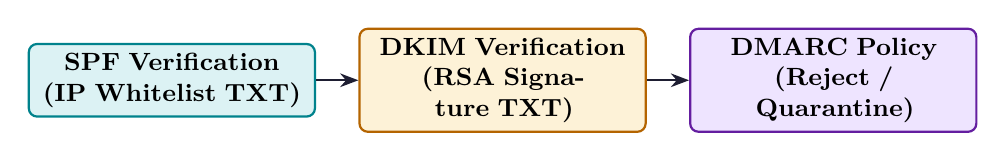
\begin{tikzpicture}[node distance=0.8cm and 1.2cm,
  spf/.style={rectangle, draw=myteal, fill=hdrteal, text width=3.4cm, align=center, minimum height=0.85cm, font=\small\bfseries, rounded corners=3pt, line width=0.8pt},
  dkim/.style={rectangle, draw=myamber, fill=hdramber, text width=3.4cm, align=center, minimum height=0.85cm, font=\small\bfseries, rounded corners=3pt, line width=0.8pt},
  dmarc/.style={rectangle, draw=mypurple, fill=hdrpurple, text width=3.4cm, align=center, minimum height=0.85cm, font=\small\bfseries, rounded corners=3pt, line width=0.8pt},
  arrow/.style={-Stealth, thick, color=mydark}]

  \node[spf] (s) at (0,0) {SPF Verification\\(IP Whitelist TXT)};
  \node[dkim] (k) at (4.2,0) {DKIM Verification\\(RSA Signature TXT)};
  \node[dmarc] (d) at (8.4,0) {DMARC Policy\\(Reject / Quarantine)};

  \draw[arrow] (s) -- (k);
  \draw[arrow] (k) -- (d);

\end{tikzpicture}
\end{tcolorbox}

\subsection{Email Protocol Mechanics}
\begin{enumerate}[leftmargin=*, itemsep=3pt]
  \item \textbf{SPF (Sender Policy Framework):} DNS record listing IP addresses authorized to send mail for a domain.
  \item \textbf{DKIM (DomainKeys Identified Mail):} Attaches an RSA digital signature to message headers, verified against the sender domain's public DNS key.
  \item \textbf{DMARC:} Evaluates SPF and DKIM alignment, instructing receiving servers how to enforce policy (`p=none`, `p=quarantine`, `p=reject`).
\end{enumerate}

\subsection{Impersonation Attacks, Malvertising \& Appropriate Use}
\begin{itemize}[leftmargin=*, itemsep=3pt]
  \item \textbf{Phishing vs Spear Phishing vs Whaling:} Broad credential harvesting emails vs customized targeted emails vs executive-targeted attacks.
  \item \textbf{Business Email Compromise (BEC):} Attackers compromise legitimate executive email accounts to order fraudulent wire transfers.
  \item \textbf{Malvertising:} Injecting malicious scripts into advertising networks to trigger drive-by malware downloads.
  \item \textbf{Appropriate Use Enforcement:} Implementing technical monitoring to ensure compliance with organization Acceptable Use Policies (AUP).
\end{itemize}

% ===============================================================================
\section{Cyber Crime, Geolocation, Privacy \& Intellectual Property Theft}
% ===============================================================================

\subsection{Geolocation \& Jurisdictional Enforcement}
Cyber crime operates borderlessly across geographical boundaries:
\begin{itemize}[leftmargin=*, itemsep=3pt]
  \item \textbf{Geo-location Tracking:} Utilizing IP geolocation databases and GPS telemetry to trace attack traffic or enforce regional content access control (geofencing).
  \item \textbf{Jurisdictional Conflict:} Attackers route malicious traffic through proxy servers across multiple foreign sovereign nations, impeding international law enforcement extradition.
\end{itemize}

\subsection{GDPR Data Privacy Principles}
The EU General Data Protection Regulation (GDPR) mandates 7 core principles:
\begin{enumerate}[leftmargin=*, itemsep=3pt]
  \item \textbf{Lawfulness, Fairness, and Transparency:} Valid consent required for processing.
  \item \textbf{Purpose Limitation:} Collecting data strictly for specified legitimate purposes.
  \item \textbf{Data Minimization:} Collecting only necessary data fields.
  \item \textbf{Accuracy:} Maintaining up-to-date accurate records.
  \item \textbf{Storage Limitation:} Deleting data when no longer required (Right to be Forgotten).
  \item \textbf{Integrity and Confidentiality:} Mandating AES encryption and breach notification within 72 hours.
  \item \textbf{Accountability:} Demonstrating continuous compliance.
\end{enumerate}

{\renewcommand{\arraystretch}{1.45}%
\begin{tabularx}{\linewidth}{|B{3.5cm}|Y|Y|}
\hline
\textbf{Cyber Crime Category} & \textbf{Modus Operandi} & \textbf{Primary Mitigation Control} \\
\hline
Financial Cyber Crime & Banking Trojans, SIM swapping, credit card skimming. & Multi-Factor Authentication (MFA), fraud monitoring. \\
\hline
Identity Theft & Stealing PII to fraudulently open accounts/loans. & Credit monitoring, Data Loss Prevention (DLP). \\
\hline
Intellectual Property Theft & Exfiltrating trade secrets, industrial designs, source code. & Data Loss Prevention (DLP), DRM encryption. \\
\hline
Ransomware & Cryptographic file locking demanding Bitcoin ransom. & Immutable offline backups, endpoint EDR agents. \\
\hline
\end{tabularx}}

\begin{tcolorbox}[examplebox, title={\textbf{Real-World Case Study: WannaCry Ransomware Pandemic (2017)}}]
\begin{enumerate}[leftmargin=*, itemsep=3pt]
  \item \textbf{Exploit Vector:} Leveraged the NSA `EternalBlue` exploit (CVE-2017-0144) targeting unpatched Microsoft Windows SMBv1 protocol.
  \item \textbf{Impact:} Encrypted 200,000+ computers across 150 countries within hours (crippling the UK NHS hospitals and FedEx).
  \item \textbf{Mitigation:} Stopped when security researcher Marcus Hutchins registered the hardcoded kill-switch domain (`iuqerfsodp9ifjaposdfjhgosurijfaewrwerg.com`).
\end{enumerate}
\end{tcolorbox}

% ===============================================================================
\section{Cyber Conflict, Espionage, Sabotage \& Warfare}
% ===============================================================================

\begin{tcolorbox}[defbox, title={\textbf{Definition: Cyber Warfare, Espionage \& Sabotage}}]
\begin{itemize}[leftmargin=*, itemsep=3pt]
  \item \textbf{Cyber Espionage:} Unauthorized covert intrusion into state or corporate networks to steal classified strategic intelligence.
  \item \textbf{Cyber Sabotage:} Deliberate destruction or physical disruption of critical physical assets using malware.
  \item \textbf{Cyber Warfare:} Nation-state cyber operations producing casualties or destruction equivalent to conventional armed attacks.
\end{itemize}
\end{tcolorbox}

\begin{tcolorbox}[examplebox, title={\textbf{Historical Case Study: Stuxnet Natanz Centrifuge Sabotage (2010)}}]
\begin{enumerate}[leftmargin=*, itemsep=3pt]
  \item \textbf{Target:} Iran's Natanz nuclear enrichment facility running Siemens S7-300 PLCs.
  \item \textbf{Vector:} Air-gapped network breached via infected USB drives using 4 Windows Zero-day exploits.
  \item \textbf{Payload:} Altered PLC rotor frequency speeds, spinning centrifuges out of control to self-destruction while sending fake normal telemetry data to monitoring consoles.
\end{enumerate}
\end{tcolorbox}

% ═══════════════════════════════════════════════════════════════════════════════
% QUICK REVISION PAGE
% ═══════════════════════════════════════════════════════════════════════════════
\newpage
\begin{center}
  {\large\bfseries\color{myred} Quick Revision --- Module 3}\\[3pt]
  {\small\color{mydark} Cyber Governance Issues, Crimes \& Conflicts $|$ OE-EC803C}
\end{center}
\noindent{\color{myred}\rule{\linewidth}{1.2pt}}
\vspace{4pt}

\begin{tcolorbox}[formulabox, title={\textbf{Key Concepts and Metrics at a Glance}}]
\renewcommand{\arraystretch}{1.35}
\begin{tabularx}{\linewidth}{B{4.8cm} X}
Email Verification Triad & SPF (IP validation), DKIM (RSA signature), DMARC (enforcement policy). \\[3pt]
DNSSEC Security & Adds cryptographic signatures (`RRSIG`) to DNS records to prevent cache poisoning. \\[3pt]
WannaCry Malware & Global ransomware spreading via EternalBlue SMBv1 exploit; stopped by kill-switch domain. \\[3pt]
Stuxnet Attack & Cyber weapon that destroyed physical Iranian nuclear centrifuges via Siemens PLCs. \\[3pt]
GDPR Breach SLA & Mandatory reporting of personal data breaches to regulators within 72 hours.
\end{tabularx}
\end{tcolorbox}

\begin{tcolorbox}[defbox, title={\textbf{One-Line Definitions}}]
\begin{itemize}[leftmargin=*, itemsep=2pt, topsep=0pt]
  \item \textbf{Net Neutrality:} Mandatory equal treatment of all web traffic without ISP throttling or fast lanes.
  \item \textbf{BEC Fraud:} Impersonating executive email accounts to order unauthorized wire transfers.
  \item \textbf{Data Sovereignty:} Laws mandating citizen data generated locally must remain within national borders.
  \item \textbf{Spear Phishing:} Highly customized phishing attack targeting a specific individual.
\end{itemize}
\end{tcolorbox}

\begin{tcolorbox}[exambox, title={\textbf{Frequently Asked / Viva Questions}}]
\begin{enumerate}[leftmargin=*, label=\textbf{Q\arabic*.}, itemsep=5pt, topsep=0pt]
  \item \Q{Define Net Neutrality and state its core rules.}
        Mandates that ISPs treat all internet traffic equally, prohibiting traffic blocking, throttling, or paid prioritization.

  \item \Q{Explain the function of SPF in email security.}
        SPF uses a DNS TXT record listing IP addresses authorized to send emails for a domain, preventing header spoofing.

  \item \Q{How does DKIM authenticate outgoing emails?}
        DKIM attaches a cryptographic digital signature to the email header; receiving mail servers verify it using the sender's public DNS key.

  \item \Q{What is DMARC and what policy actions does it mandate?}
        DMARC checks SPF and DKIM alignment, instructing receiving servers to enforce `none`, `quarantine`, or `reject` policies on invalid emails.

  \item \Q{Describe the WannaCry ransomware pandemic.}
        WannaCry infected 200,000+ computers across 150 countries by exploiting the SMBv1 `EternalBlue` vulnerability, encrypting hard drives for Bitcoin ransom.

  \item \Q{Explain the significance of the Stuxnet worm.}
        Stuxnet was the first cyber weapon to cause physical infrastructure destruction, ruining 1,000+ Iranian nuclear centrifuges via Siemens PLCs.

  \item \Q{What is Business Email Compromise (BEC)?}
        A social engineering fraud scheme where attackers compromise or spoof executive email accounts to trick financial staff into executing wire transfers.

  \item \Q{How does DNSSEC prevent DNS Cache Poisoning?}
        By signing DNS resource records with cryptographic keys (`RRSIG`), ensuring clients verify DNS response integrity before caching.

  \item \Q{What are the 7 core principles of GDPR?}
        Lawfulness, Purpose Limitation, Data Minimization, Accuracy, Storage Limitation, Integrity \& Confidentiality, and Accountability.

  \item \Q{What is Data Sovereignty?}
        The legal requirement that digital data created within a country must be subject to that nation's laws and stored within its physical boundaries.

  \item \Q{Define Malvertising.}
        Injecting malicious advertisements into legitimate ad networks to infect users via silent drive-by downloads without clicking.

  \item \Q{What is the role of ICANN in internet governance?}
        Managing global IP address allocation (IPv4/IPv6 via IANA), coordinating DNS root zone servers, and managing top-level domain (TLD) registries.

  \item \Q{Differentiate between Cyber Espionage and Cyber Sabotage.}
        Cyber Espionage focuses on secret intelligence gathering; Cyber Sabotage focuses on physical or operational system destruction.

  \item \Q{Explain the term 'Drive-by Download'.}
        Malware installation that occurs automatically upon visiting a compromised website without explicit user download consent.

  \item \Q{What is the GDPR breach notification timeframe?}
        Data controllers must notify relevant data protection authorities within 72 hours of becoming aware of a personal data breach.
\end{enumerate}
\end{tcolorbox}

\begin{tcolorbox}[tikzbox, title={Summary Comparison: Email Authentication Protocols}]
\centering
{\renewcommand{\arraystretch}{1.45}%
\begin{tabularx}{\linewidth}{|B{2.2cm}|Y|B{3.8cm}|Y|}
\hline
\textbf{Protocol} & \textbf{Verification Mechanism} & \textbf{DNS Record Type} & \textbf{Primary Defense Focus} \\
\hline
SPF & Validates Sending Mail Server IP & TXT (`v=spf1`) & Sender Address Spoofing \\
\hline
DKIM & Validates Cryptographic RSA Header & TXT (`selector.\_domainkey`) & Message Header Tampering \\
\hline
DMARC & Enforces Policy Alignment (`p=reject`) & TXT (`\_dmarc`) & Phishing \& Unauthenticated Delivery \\
\hline
\end{tabularx}}
\end{tcolorbox}

\end{document}
